\subsection{\label{sec:spatial_structure_of_neural_systems}Spatial Structure of Neural Systems}
The core principle behind the ability of neural systems to efficiently move information across space is that networks are comprised of specialized modules arranged in a hierarchical configuration. This modular and hierarchical architecture repeats in a self-similar manner from the scale of neurons up to the scale of the system as a whole. To understand these spatial principles quantitatively, we begin by summarizing the relevant concepts from graph theory \cite{eskn2015}.

\vspace{1em}
consider beginning with a brief description of what aspects of brain anatomy we're discussing (synapses, dendrites, soma, axons, mini-columns, columns, areas, sheet of cortex, other brain structures, thalamus, hippocampus)

\subsubsection{Adjacency matrix}
In order for the neurons to differentiate their responses while efficiently exchanging information across the network, certain structural network considerations are pertinent \cite{rusp2010}. The structures of neural systems are analyzed in the framework of network theory \cite{eskn2015}. In network theory, a system is discussed as a set of nodes connected by a set of edges. To facilitate mathematical analysis, the system is represented by an adjacency matrix, $\mathbf{A}$. Each column of $\mathbf{A}$ represents a node in the network, and if an edge connects node $i$ to node $j$, $A_{ij} = 1$, otherwise $A_{ij} = 0$. Connections can be directed, in which case $\mathbf{A}$ will be, in general, non-symmetric. Connections can also we weighted, in which case the adjacency matrix becomes a weight matrix, $\mathbf{W}$, whose elements represent not only the presence of edges, but also their strength.

To analyze a network, we label each node with an index $1\le i\le N$, where $N$ is the total number of nodes in the network. If we know all the connections between the nodes in the network, we can proceed to construct the adjacency matrix. In neural systems, we may use network theory to analyze the system at various scales. At the smallest (device) scale, each neuron may be represented a node, and each synapse by a directed edge. Alternatively, at the system scale, brain regions may be represented by nodes and the connections between these regions by edges. Across these scales, certain network metrics are important for analyzing performance. 

\subsubsection{Node Degree and Degree Distribution}
A simple yet important quantity that can be calculated from the adjacency matrix is the number of connections made by each node. If the network has directed connections, the number of outgoing edges (out-degree) will, in general, be different from the number of incoming edges (in-degree). The out-degree is given by $k^{\mathrm{out}}_i = \sum_jA_{ij}$, and the in-degree is given by $k^{\mathrm{out}}_j = \sum_iA_{ij}$. At the scale of devices, the in-degree represents the number of synaptic connections terminating on a given neuron, and the out-degree represents the number of synaptic connections made by a given neuron. The function describing the degrees of all nodes in network is referred to as the degree distribution.

\subsubsection{Path Length}
One reason the node degree is important is that it enables us to calculate the average minimum path length across the network. To calculate this quantity, we find the minimum path length (number of edges that must be traversed) for each pair of nodes in the network, and we take the average over all pairs. This average minimum path length is a coarse, global metric that provides information regarding the ability of information to be efficiently exchanged across the network. In constructing a neural system, one would like to keep path lengths as short as possible to facilitate efficient communication from any neuron to any other neuron. In general, network path lengths are minimized in random networks \cite{baal1999}, wherein edges between nodes are assigned at random. Therefore, by considering the average minimum path length of a random network, we can estimate the connectivity required between neurons in order to maintain efficient communication across a neural system of a given size. This average path length can be calculated in closed form \cite{frfr2004}. This quantity is plotted in Fig.\,\ref{fig:data}(a), where we show the number of edges required per node ($\bar{k}$) to achieve a given average path length ($\bar{L}$) as a function of the number of nodes in the network \cite{frfr2004}. Consider the case of a network with one million nodes. We see from this plot that if we wish to maintain a path length of two, each node must make, on average, one thousand connections. For the case of a network with 100 million nodes, each node must make 10,000 connections. This is similar to the case of the hippocampus in the human brain, with nearly 100 million neurons, each with 10,000 or more synaptic connections \cite{bu2006}. Maintaining a short average path length across the network is critical to enable efficient information integration, and this appears to be a major factor driving the extensive connectivity of biological neural systems, and our design of neural hardware for cognition must account for the requirement of many connections to enable efficient communication across the network.  
\begin{figure} 
    \centering{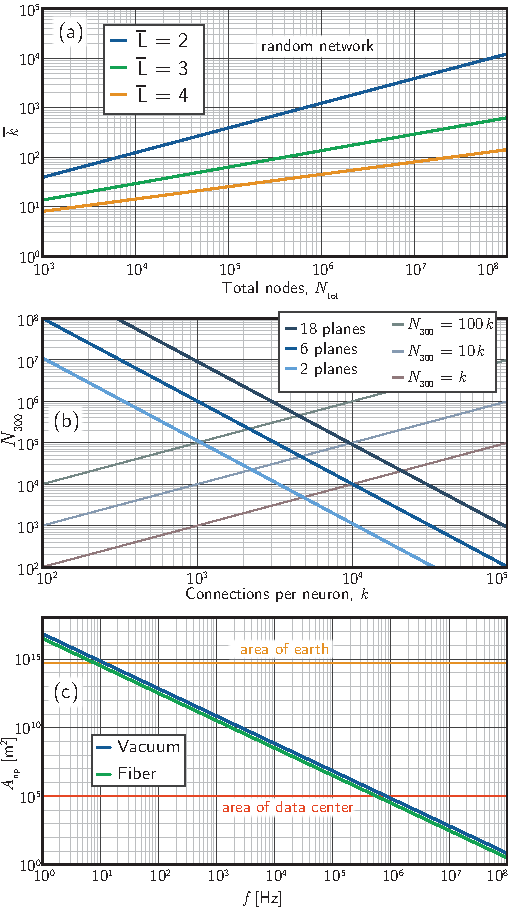
\includegraphics[width=8.6cm]{data_plots.pdf}}
	\captionof{figure}{\label{fig:data}Scaling considerations for optoelectronic neural systems. (a) The average number of connections per node required to maintain a give average path length across a random network as a function of the total number of nodes in the system. (b) The total number of nodes that can fit on a 300\,mm wafer as a function of the number of connections per node in the wire-limited regime \cite{ke1982}. (c) The area of the neuronal pool as a function of the frequency of neuronal oscillations assuming light-speed communication \cite{shICRC2018}.}
\end{figure}

\subsubsection{Clustering}
This analysis of average path length is relevant for quantifying a network's potential for information integration, but as we stated above, a neural system also depends on the ability for differentiated processing. Let us consider differentiation across various scales of the network. Ideally, no two neurons would behave identically, because this would not provide new information. Each neuron will fire preferentially in response to stimulus according to a tuning curve \cite{daab2001}. In practice, some redundancy is advantageous if a network is to rapidly gain confidence regarding the nature of a stimulus. Neural systems employ populations of neurons to represent certain pieces of information. The net activity across the population represents the presence or absence of a stimulus, and the variation in activity across the population represents uncertainty about the interpretation of the stimulus. In order for a certain population of neurons to predominantly exchange information locally and rapidly establish a consensus interpretation of a stimulus, the neurons in that population should comprise a preponderance of connections within the population. Groups of neurons with an abundance of connections within the group relative to connections external to the group form a community, and a clustering coefficient \cite{eskn2014,fa2007} is the simplest network metric. If node $a$ is connected to node $b$ and to node $c$, the clustering coefficient quantifies the fraction of cases in which node $b$ is also connected to node $c$. This metric provides insight into the tendency of neurons to form specialized communities with information processing differentiated from other parts of the network, and is first step toward analyzing the modularity of the system. 

\subsubsection{Small-World Networks}
A random network has a low clustering coefficient, as the presence or absence of a connection between nodes $b$ and $c$ is, by definition, completely independent of the presence or absence of any connections to or from node $a$. Yet the networks of the brain\textemdash from the scale of neurons to the scale of connections between regions\textemdash show a high degree of clustering relative to a random network. As we have emphasized, neural information processing relies on both differentiated processing by local clusters and efficient integration of information across the network. We therefore expect neural systems to simultaneously achieve a high clustering coefficient and short average path length. A small-world networks is one with both of these traits \cite{wast1998}. We can introduce the small-world index (SWI) \cite{hugu2008} given by  $\mathrm{SWI} = \frac{\bar{C}/\bar{L}}{\bar{C}_{\mathrm{r}}/\bar{L}_{\mathrm{r}}}$, where $\bar{C}$ is the average clustering coefficient, $\bar{L}$ is the average shortest path, and the subscript, $\mathrm{r}$, refers to a random graph. Whether analyzed at the scale of populations of a few thousand neurons or at the scale of large regions of the brain, the networks demonstrate large $\mathrm{SWI}$, indicating that different populations of neurons represent different information, the activities of these populations can be efficiently communicated across the network, and  giving hints that brain architecture is hierarchical and modular.

\subsubsection{\label{sec:modularity_and_hierarchy}Modularity and Hierarchy}
Anatomically, clusters in the brain were thoroughly described by Mountcastle in 1977 \cite{mo1978} before the concept of a small-world network had been introduced \cite{wast1998}. Mountcastle referred to the communities of neurons as mini-columns and columns. Imaging of biological neural systems with various techniques across all relevant length scales indicates modularity persists across multiple levels of hierarchy \cite{beba2017}. The clustering coefficient discussed above can be generalized to the modularity, $Q$, quantifying the degree to which the connections of a network depart from what would be expected of a random network to form partitioned communities \cite{rusp2010,beba2017}. For example, clusters of neurons are partitioned into mini-columns. At the next level of hierarchy, clusters of mini-columns are partitioned into columns. Clusters of columns are partitioned into brain regions. At the highest level of hierarchy in the brain, regions exchange information throughout the cerebral cortex and the thalamocortical complex that controls and coordinates operation of the largest modules comprising the brain \cite{bosp2015}. Neurons predominantly contribute to activity within their module, but they also must be able exchange information across partitions and up the information-processing hierarchy. Again we find differentiated, local processing combined with information integration across the hierarchical structure of the network. This neural information processing is enabled by a small-world architecture.



(probably need more here. make sure it is well set up for neuronal avalanches section and fractal use of space and time. define modular and hierarchical)

As Simon argued in 1962, `` Hierarchy...is one of the central structural schemes that the architect of complexity uses.'' \cite{si1962}. Modular and hierarchical architectures are the foundation of nearly all complex structures and systems. 

A \textbf{\textit{hierarchic system}} is ``a system that is composed of interrelated subsystems, each of the latter being, in turn, hierarchic in structure until we reach some lowest level of elementary subsystem.'' \cite{si1962}

``I shall use hierarchy in the broader sense...to refer to all complex systems analyzable into successive sets of subsystems.'' \cite{si1962}

``...we can distinguish between the interactions \textit{among} subsystems, on the one hand, and the interactions \textit{within} subsystems\textemdash i.e., among the parts of those subsystems\textemdash on the other.'' \cite{si1962}

``Empirically, a large proportion of the complex systems we observe in nature exhibit hierarchic structure. On theoretical grounds we could expect complex systems to be hierarchies in a world in which complexity had to evolve from simplicity.'' \cite{si1962} This tendency to observe hierarchical configuration in complex systems results from several factors, including the requirement of manufacturability (even in non-artificial systems such as life forms) and the efficiency resulting from the ability to optimize a small number of components and nearly independently optimize their configuration and interaction within the context of the system.

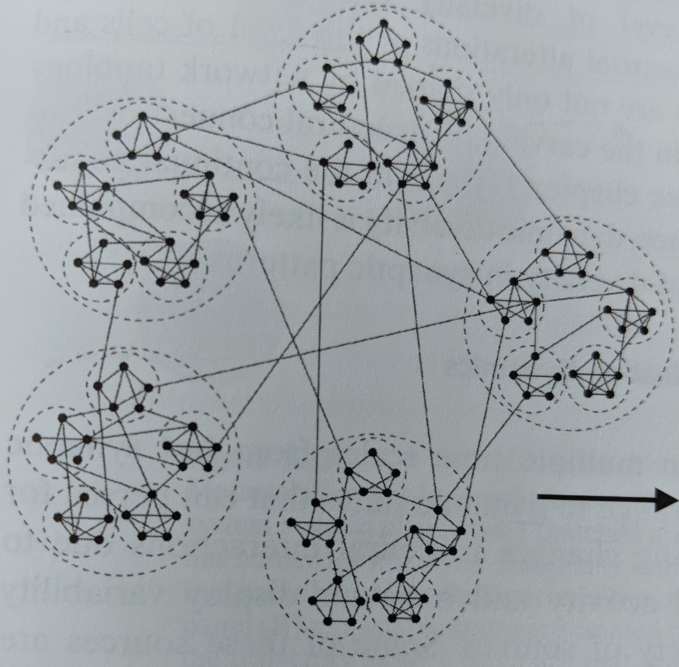
\includegraphics[width=8.6cm]{figures/_sporns_hierarchical_modularity.png}
\captionof{figure}{\label{fig:sporns_hierarchical_modularity}Schematic of a modular, hierarchical network. From Ref.\,\onlinecite{sp2010}, pg. 261.}

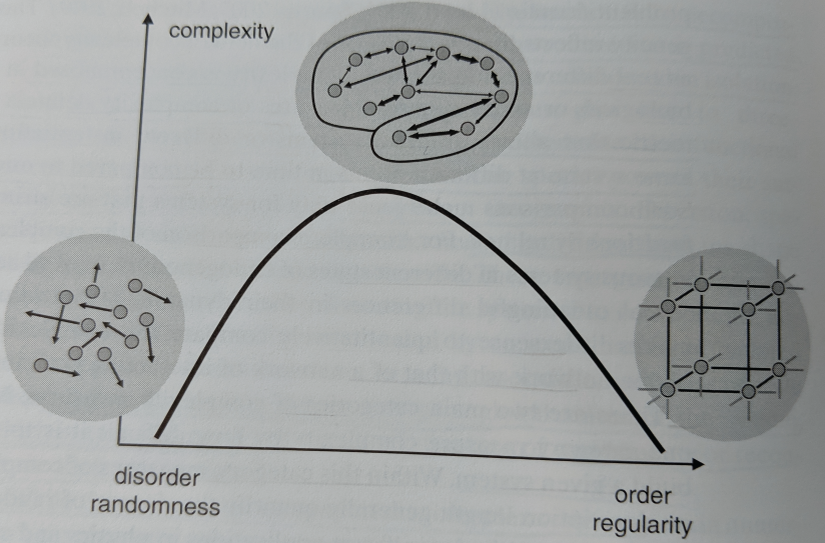
\includegraphics[width=8.6cm]{figures/_sporns_complexity.png}
\captionof{figure}{\label{fig:sporns_complexity}Schematic of complexity as a balance of order and disorder. From Ref.\,\onlinecite{sp2010}, pg. 282.}

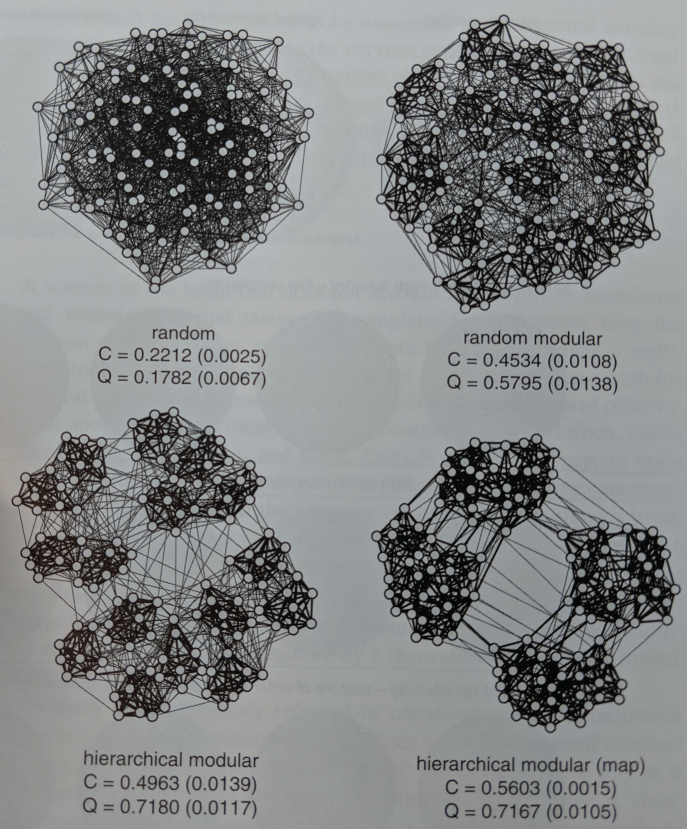
\includegraphics[width=8.6cm]{figures/_sporns_complexity_and_hierarchical_modularity.png}
\captionof{figure}{\label{fig:sporns_complexity_and_hierarchical_modularity}Complexity and hierarchical modularity. From Ref.\,\onlinecite{sp2010}, pg. 291.}

\vspace{1em}
emphasize that hierarchy is defined by connections and exists even in the unform, 2D sheet of the cortex.

\subsubsection{Rentian Analysis}
%\begin{figure} 
%    \centering{\includegraphics[width=8.6cm]{rentian_analysis.pdf}}
%	\captionof{figure}{\label{fig:rentian_analysis}Caption.}
%\end{figure}
We can quantify the ability of information to be communicated up the hierarchy by analyzing the number of connections penetrating various partitions of the network, referred to as Rentian analysis. Rent's rule states that the number of edges crossing the boundary of a partition ($k$) is related to the number of nodes within the partition ($n$) by a power law of the form
\begin{equation}
\label{eq:Rent}
\varepsilon = \varepsilon_1 n^p,
\end{equation}
where $\varepsilon_1$ is the number of edges emanating from each node (first level of hierarchy), and $p$ is referred to as the Rent exponent. Rent's rule (Eq.\,\ref{eq:Rent}) was first observed in the context of VLSI circuits, and has also been shown to hold for biological neural circuits ranging from \textit{C. elegans} to the human brain \cite{bagr2010}. 

Depending on the system under study, the Rent exponent may vary, but is generally around 0.75 \cite{bagr2010}. We will demonstrate the use of Eq.\,\ref{eq:Rent} in Sec.\,\ref{sec:scaling}. The significance of the Rent exponent can be seen in its relation to the topological dimension, $D$. In Euclidean geometry, the surface area of a structure embedded in $d$-dimensional space is given by a power law of the form $s\sim v^p$. In general, the surface area $s$ scales as a length to the power of $d-1$, while the volume scales as a length to the power of $d$. Thus, in Euclidean geometry, $p = 1-1/d$, or $d = (1-p)^{-1}$. The same expression holds in fractal geometry \cite{ma1983,sc1991}, and in the case of Rentian scaling the topological dimension is related to the Rent exponent by $D = (1-p)^{-1}$, with $0 \le p \le 1$, so that $1 \le D \le \infty$. For $p > 2/3$, the topological dimension is larger than the embedding dimension, indicating that through a judicious implementation of input and output ports, information can flow through a network as if its components were connected in a higher-dimensional space. In the case of the brain, we find $D \approx 4$.

In any real network, it will only be possible to adhere to Eq.\,\ref{eq:Rent} across a certain domain of $n$. In the brain, consideration can apply from a single neuron up to the brain as a whole. Yet across this domain, Eq.\,\ref{eq:Rent} applies only piecewise, with discontinuities at certain partitions \cite{oz2004}. For example, we may expect Eq.\,\ref{eq:Rent} to hold from the scale of a single neuron up to the scale of a cortical column, but the connectivity patterns between columns are quite different than within, so we may expect a discontinuity at the scale of cortical columns, followed by a new expression of Eq.\,\ref{eq:Rent} with a different value of $p$, and perhaps a new interpretation of $n$ as the number of columns within a partition. Similarly in the domain of microelectronics, a multicore processor on a chip may obey Eq.\,\ref{eq:Rent} within each processor, with a discontinuity at the scale of the connections between processors. The wiring organization of VLSI circuits and the brain is statistically fractal, but not infinitely so. The limitations are purely physical.  

How does Rentian analysis inform our design of neural hardware? As we have emphasized, neural information is processed across a modular hierarchy. Rentian analysis quantifies the ability of information to be transmitted across partitions in the hierarchy. We conjecture that the ability for a neural system transmit more information across more levels of hierarchy will improve general intelligence. Therefore, between the neurons within a module, we expect that neural hardware should achieve high values of $D$ over a large range of $n$ before a discontinuity is necessary, so that multiple levels of hierarchy can be traversed efficiently within a module. Further, upon encountering a discontinuity, hardware must have a means of establishing another domain of Rentian scaling to efficiently collect and distribute information across more orders of hierarchy. Finally, we conjecture that the most intelligent neural hardware will provide this fractal scaling across as many levels of hierarchy as possible until the system finally reaches the limits set by the speed of communication. In Sec.\,\ref{sec:scaling} we will discuss these large-scale limits in biological and optical systems.

\subsubsection{Summary of Spatial Considerations}
The spatial structure of a neural system must comprise nodes with many edges to enable short path length across large networks. These nodes must also have high clustering to enable differentiated processing within modules. The information from these modules must be integrated across the hierarchy of the network, and the ability to do so is quantified by the topological dimension. Neural systems efficiently process information through the fractal use of space. Let us now consider their operation in time.